\documentclass[../main.tex]{subfiles}
\begin{document}

    \section{Persona Survey Questions}

    The Word and PDF versions of the persona survey can be found here:
    \url{https://github.com/chendaniely/dissertation-irb/tree/master/irb-20-537-data\_science\_workshops/survey}.
    The survey is listed as ``survey-01-pre\_workshop\_self\_assessment''.

    \section{Persona Occupation}

        The occupation question for the persona survey had a few options participants can check off.
        They are able to check off all the occupations that applied to themselves and were also able to write in their own option.

        \begin{figure}[htb]
            \centering
            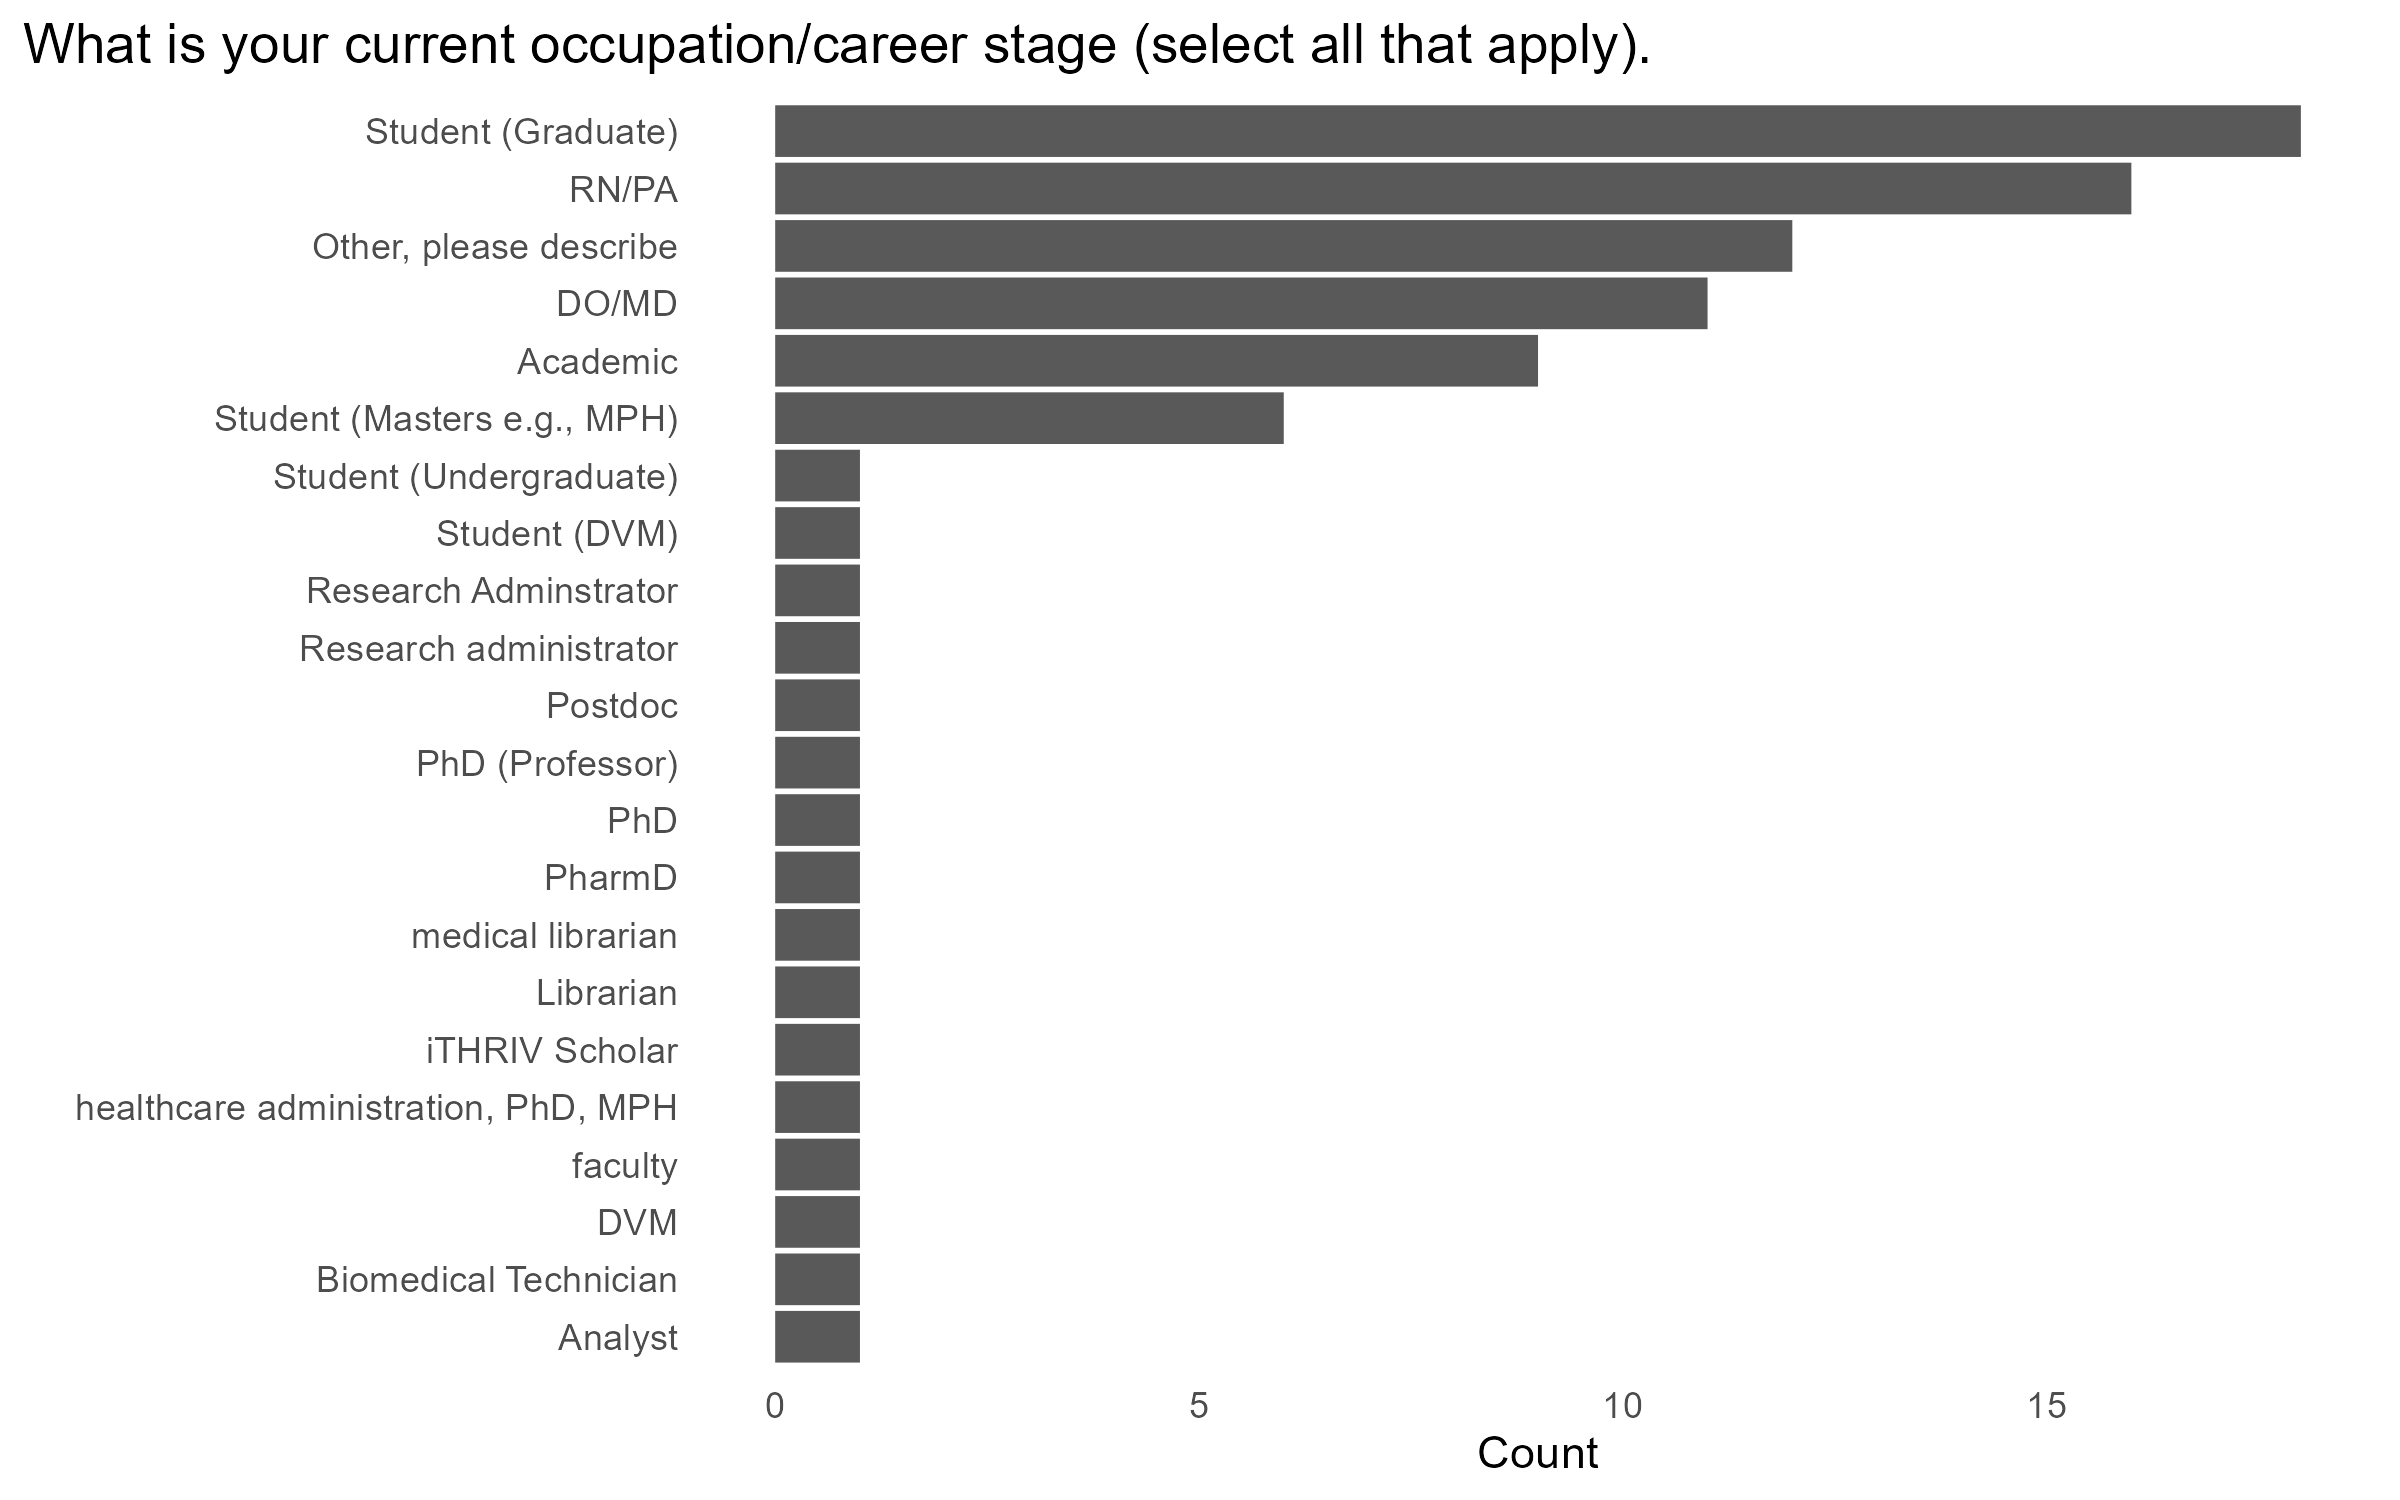
\includegraphics[width=0.7\linewidth]{figs/020-persona/Q2.3.png}
            \caption[What is your current occupation/career stage (select all that apply)]
            {Self reported current occupation and career stage.
                Respondents are able to select multiple options and also write in their own choices.
            }
            \label{fig:demographics_occupation}
        \end{figure}

        \begin{figure}[htb]
            \centering
            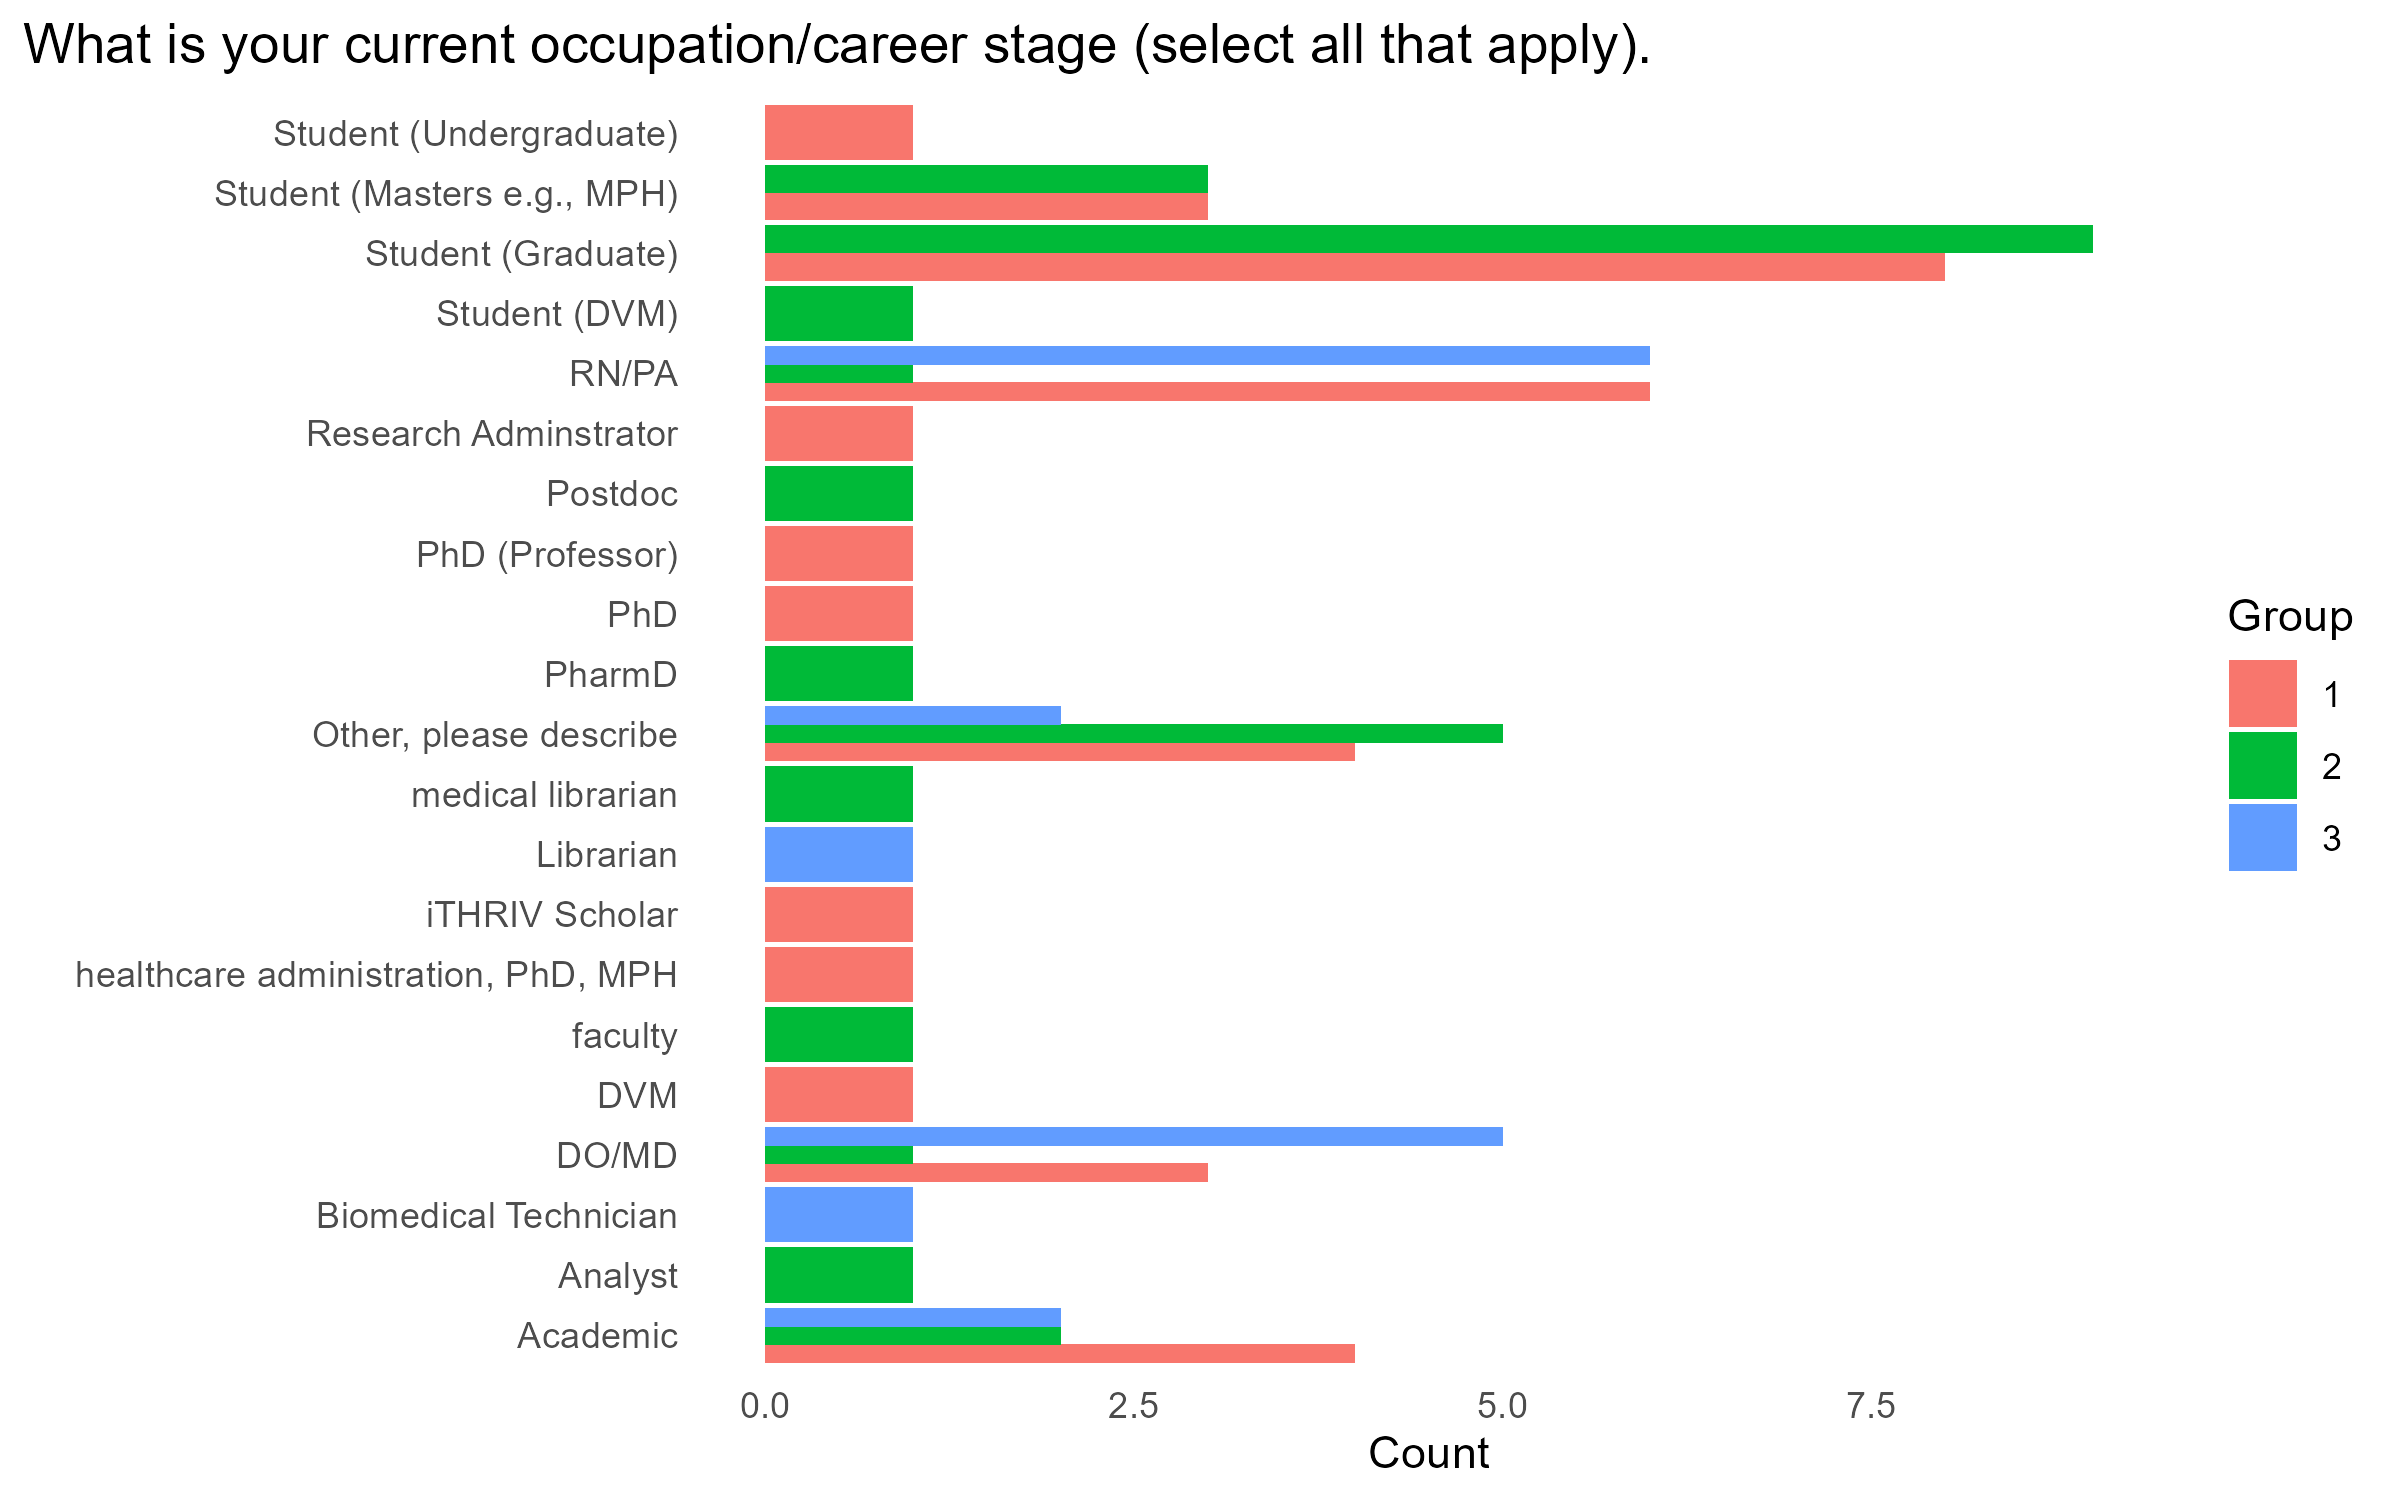
\includegraphics[width=0.7\linewidth]{figs/020-persona/survey\_likert/Q2.3-group-3.png}
            \caption[What is your current occupation/career stage by group (select all that apply)]
            {Self reported current occupation and career stage by clustering group.
                Respondents are able to select multiple options and also write in their own choices.
            }
            \label{fig:demographics_occupation_cluster}
        \end{figure}

    \section{Factor Analysis}

        \begin{figure}[htb]
            \centering
            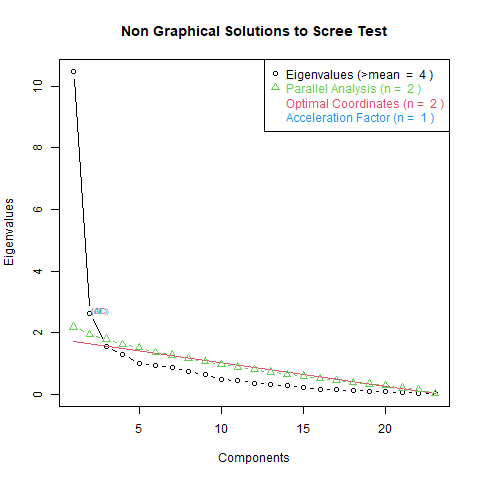
\includegraphics[scale=0.5]{figs/010-validation/efa_eigen_scree.png}
            \caption[Scree plot for factor analysis]
            {Scree plot for factor analysis showing the number of components (x) and the eigenvalues (y).
                The figure suggests exploring 2 to 4 factor models.
            }
            \label{fig:scree-fa-all}
        \end{figure}

        \subsection{Data normality}
        \label{ss:fa-data-normality}

            Looked at histograms and qqplots.
            Also looked at Shapiro Wilk's test for normalality.

    % https://m-clark.github.io/posts/2020-04-10-psych-explained/
    % https://m-clark.github.io/posts/2020-04-10-psych-explained/

%    h2: the amount of variance in the item/variable explained by the (retained) factors. It is the sum of the squared loadings, a.k.a. communality.
%    u2: 1 - h2. residual variance, a.k.a. uniqueness
%    com: Item complexity. Specifically it is “Hoffman’s index of complexity for each item. This is just (Σλ2i)2/Σλ4i
%    where λi is the factor loading on the ith factor. From Hofmann (1978), MBR. See also Pettersson and Turkheimer (2010).” It equals one if an item loads only on one factor, 2 if evenly loads on two factors, etc. Basically it tells you how much an item reflects a single construct. It will be lower for relatively lower loadings.

        \subsection{2 Factor Model}

            % latex table generated in R 4.1.1 by xtable 1.8-4 package
            % Mon Oct 18 13:21:20 2021
            \begin{table}[ht]
                \centering
                \begin{tabular}{rlllrrr}
                    \hline
                    & item & MC1 & MC2 & Communality & Uniqueness & Complexity \\
                    \hline
                    1 & Q3.3 & 0.902 &  & 0.88 & 0.12 & 1.15 \\
                    2 & Q3.5 & 0.896 &  & 0.86 & 0.15 & 1.12 \\
                    3 & Q3.4 & 0.894 &  & 0.82 & 0.18 & 1.06 \\
                    4 & Q3.1 & 0.884 &  & 0.81 & 0.16 & 1.14 \\
                    5 & Q7.2\_2 & 0.876 &  & 0.82 & 0.16 & 1.18 \\
                    6 & Q7.2\_5 & 0.802 & 0.311 & 0.75 & 0.26 & 1.29 \\
                    7 & Q7.2\_4 & 0.737 &  & 0.58 & 0.40 & 1.21 \\
                    8 & Q7.2\_6 & 0.728 &  & 0.54 & 0.46 & 1.03 \\
                    9 & Q5.2 & 0.707 & 0.341 & 0.58 & 0.38 & 1.44 \\
                    10 & Q7.2\_7 & 0.66 &  & 0.44 & 0.56 & 1.01 \\
                    11 & Q4.3 & 0.636 &  & 0.43 & 0.58 & 1.09 \\
                    12 & Q7.2\_3 & 0.634 & 0.321 & 0.48 & 0.49 & 1.48 \\
                    13 & Q4.4 & 0.468 &  & 0.28 & 0.74 & 1.34 \\
                    14 & Q4.2 & 0.46 & 0.442 & 0.44 & 0.59 & 2.00 \\
                    15 & Q3.7 &  &  & 0.02 & 0.93 & 1.77 \\
                    16 & Q6.2 &  & 0.914 & 0.84 & 0.12 & 1.10 \\
                    17 & Q6.1 &  & 0.9 & 0.88 & 0.11 & 1.19 \\
                    18 & Q6.3 &  & 0.804 & 0.71 & 0.29 & 1.18 \\
                    19 & Q3.6 &  & 0.54 & 0.35 & 0.70 & 1.08 \\
                    20 & Q6.4 & 0.341 & 0.435 & 0.33 & 0.69 & 1.89 \\
                    21 & Q4.1 &  & 0.418 & 0.17 & 0.81 & 1.12 \\
                    22 & Q7.2\_1 &  & 0.342 & 0.10 & 0.88 & 1.00 \\
                    23 & Q5.1 &  &  & 0.05 & 0.96 & 1.49 \\
                    \hline
                \end{tabular}
            \end{table}

        \subsection{4 Factor Model}

            % latex table generated in R 4.1.1 by xtable 1.8-4 package
            % Mon Oct 18 13:22:58 2021
            \begin{table}[ht]
                \centering
                \begin{tabular}{rlllllrrr}
                    \hline
                    & item & MC1 & MC2 & MC3 & MC4 & Communality & Uniqueness & Complexity \\
                    \hline
                    1 & Q3.3 & 0.891 &  &  &  & 0.95 & 0.05 & 1.42 \\
                    2 & Q7.2\_2 & 0.888 &  &  &  & 0.87 & 0.12 & 1.22 \\
                    3 & Q3.4 & 0.883 &  &  &  & 0.86 & 0.14 & 1.21 \\
                    4 & Q3.5 & 0.882 &  &  &  & 0.86 & 0.14 & 1.23 \\
                    5 & Q3.1 & 0.865 &  &  &  & 0.82 & 0.17 & 1.23 \\
                    6 & Q7.2\_5 & 0.848 & 0.329 &  &  & 0.91 & 0.09 & 1.54 \\
                    7 & Q7.2\_4 & 0.754 &  &  &  & 0.72 & 0.29 & 1.53 \\
                    8 & Q5.2 & 0.716 & 0.332 &  &  & 0.63 & 0.37 & 1.45 \\
                    9 & Q4.3 & 0.604 &  &  &  & 0.44 & 0.56 & 1.42 \\
                    10 & Q7.2\_3 & 0.596 &  &  &  & 0.58 & 0.46 & 2.09 \\
                    11 & Q4.4 & 0.458 &  &  &  & 0.30 & 0.72 & 1.72 \\
                    12 & Q4.2 & 0.441 & 0.401 &  &  & 0.40 & 0.60 & 2.49 \\
                    13 & Q6.2 &  & 0.901 &  &  & 0.91 & 0.08 & 1.26 \\
                    14 & Q6.1 &  & 0.864 &  &  & 0.86 & 0.13 & 1.34 \\
                    15 & Q6.3 &  & 0.766 &  &  & 0.74 & 0.26 & 1.56 \\
                    16 & Q3.6 &  & 0.534 &  &  & 0.32 & 0.64 & 1.54 \\
                    17 & Q6.4 & 0.376 & 0.447 &  &  & 0.40 & 0.65 & 2.04 \\
                    18 & Q4.1 &  & 0.425 &  &  & 0.22 & 0.80 & 1.21 \\
                    19 & Q7.2\_7 & 0.537 &  & 0.751 &  & 0.92 & 0.06 & 2.16 \\
                    20 & Q7.2\_6 & 0.621 &  & 0.707 &  & 0.95 & 0.04 & 2.26 \\
                    21 & Q7.2\_1 &  & 0.309 & 0.332 &  & 0.33 & 0.79 & 2.13 \\
                    22 & Q3.7 &  &  &  &  & 0.05 & 0.85 & 1.70 \\
                    23 & Q5.1 &  &  &  &  & 0.25 & 0.91 & 2.20 \\
                    \hline
                \end{tabular}
            \end{table}

        \section{Factor Analysis on subset data}

            % latex table generated in R 4.1.1 by xtable 1.8-4 package
            % Sun Oct 24 23:50:35 2021
            \begin{table}[ht]
                \centering
                \begin{tabular}{rllllrrr}
                    \hline
                    & item & MC2 & MC1 & MC3 & Communality & Uniqueness & Complexity \\
                    \hline
                    1 & Q3.3 & 0.861 & 0.329 & 0.317 & 0.95 & 0.05 & 1.58 \\
                    2 & Q3.4 & 0.796 & 0.31 & 0.342 & 0.84 & 0.15 & 1.69 \\
                    3 & Q3.5 & 0.776 & 0.336 & 0.387 & 0.87 & 0.14 & 1.88 \\
                    4 & Q3.1 & 0.693 & 0.374 & 0.462 & 0.81 & 0.17 & 2.35 \\
                    5 & Q5.2 & 0.61 &  & 0.479 & 0.60 & 0.38 & 2.03 \\
                    6 & Q4.2 & 0.478 &  &  & 0.44 & 0.68 & 1.74 \\
                    7 & Q4.3 & 0.416 & 0.391 & 0.349 & 0.46 & 0.55 & 2.94 \\
                    8 & Q7.2\_7 &  & 0.931 &  & 0.96 & 0.04 & 1.22 \\
                    9 & Q7.2\_6 & 0.304 & 0.887 &  & 0.96 & 0.04 & 1.45 \\
                    10 & Q7.2\_5 & 0.506 &  & 0.703 & 0.79 & 0.17 & 2.17 \\
                    11 & Q7.2\_4 & 0.407 & 0.333 & 0.659 & 0.68 & 0.29 & 2.21 \\
                    12 & Q7.2\_2 & 0.601 & 0.323 & 0.658 & 0.90 & 0.10 & 2.46 \\
                    13 & Q7.2\_3 & 0.389 & 0.389 & 0.48 & 0.62 & 0.47 & 2.87 \\
                    \hline
                \end{tabular}
            \end{table}

    \section{Clustering}

        \begin{figure}[htb]
            \centering
            \includegraphics[width=0.7\linewidth]{figs/020-persona/survey\_likert/dendogram\_3.png}
            \caption[3 cluster dendrogram.]
            {Dendrogram showing 3 clusters
            }
            \label{fig:dendro-3}
        \end{figure}

        \begin{figure}[htb]
            \centering
            \includegraphics[width=0.7\linewidth]{figs/020-persona/survey\_likert/dendogram\_4.png}
            \caption[4 cluster dendrogram.]
            {Dendrogram showing 4 clusters
            }
            \label{fig:dendro-4}
        \end{figure}

    \section{Learner Personas}
    \label{se:learner-personas}

        We identified 3 learner personas in our group.
        The final persona, Patricia Programmer,
        was dropped from the personas when more data was collected.

        \subsection{Alex Academic}

            Alex, a professor of bioinformatics,
            studies molecular dynamics of proteins and protein-protein interactions.
            They are also responsible for teaching an introductory research class to 100 freshman and sophomore students every year.
            They also run a data consulting service at their university,
            providing support for data-related challenges to research and instructors from any discipline.

            Students complain that intro courses in programming are too theoretical and require more programming knowledge than they have.
            Many students in the department also cannot register for similar classes
            Alex, has 10s of students working for them in computational molecular dynamics simulations and other data analytics projects.

            \subsubsection{Relevant prior knowledge or experience}

                Alex performs their research using a combination of
                Excel spreadsheets and specialized software,
                but is switching to R or Python (which they taught themselves during a sabbatical).
                They have never taken a formal programming course,
                and suffers from impostor syndrome in discussions about programming.
                Alex would like to learn more about how programming can help their research and
                keep up with the tools their students are learning in class.

            \subsubsection{Perception of needs}

                Alex needs workshops (so they can allocate focused time)
                and how-to guides (for research).
                They would like ready-to-use lesson material that could be remixed for their students and
                some orientation material to demystify jargon (what is “tidy data”?).
                Alex also wants to be able to use the same tools in their research
                as in their teaching to amortize learning costs and stay in practice.

            \subsubsection{Special considerations}

                Alex wants to provide technical training to students,
                but does not have the actual time to teach all the relevant skills.
                As a person in STEM,
                they typically find themselves isolated and alone when taking formal technical classes and
                is scared to appear ignorant, and are reluctant to speak up and ask questions.


        \subsection{Clare Clinician}

            Clare has spent the last 6 years working in the Cardiothroasic ICU in a large medical hospital system.
            They read lots of gushing articles about data science,
            and was excited by the prospect of learning how to do it,
            but nothing makes sense when trying to learn it on their own.
            Clare has always been a good student and always excelled at things they tried to learn;
            they are hard on themselves when struggling to learn a new skill and
            would rather place blame on the long hours at work than having their peers know they could use assistance.

            \subsection{Relevant prior knowledge or experience}

                Clare keeps up with medical research,
                but has little to no experience in doing medical research.
                They use Excel for non-data related tasks (e.g., making lists),
                or manually inputting patient data into spreadsheets for chart reviews.
                Clare wants to be able to collect and manage data as well as
                learn about the process behind data analysis to perform their own analysis and study one day.

            \subsection{Perception of needs}

                Clare wants self-paced tutorials with practice exercises,
                plus forums where they can ask for help.
                They also need short overviews to orient them and
                introductory tutorials that include videos or animated GIFs showing exactly how to drive the tools,
                and that use datasets they can relate to.
                Clare wishes they had a community of other people in
                the medical field who are interested in learning how to do data work so they can learn and ask questions.

            \subsection{Special considerations}

                Clare is a single parent who juggle their time at work and at home who are strapped for time to learn a new skill.

        \subsection{Samir Student}

            Samir is a graduate student in a bioinformatics program.
            They worked in a wet lab doing bench since their undergraduate days studying neuroscience.
            These days Samir is doing more computational work and
            starting to use programming based tools to look at protein structures.
            They’ve taken a few classes that had had programming based homework assignments and projects,
            but the lectures themselves were mostly around theory, and many of the programming skills were self-taught.

            \subsubsection{Relevant prior knowledge or experience}

                Samir is fairly proficient in Excel and
                does works with spreadsheets regularly and
                knows how to load up Excel spreadsheets into R and do basic data processing and analysis.
                However,
                they do not have that much practice outside of a classroom homework and project setting,
                and spends a lot of their time on StackOverflow copying and pasting code
                so they don’t consider themselves a ``real programmer''.
                They have no problem getting their work done, but usually involves a lot of googling to eventually get the solution.

            \subsubsection{Perception of Needs}

                Samir wants a formal workshop and reference materials
                that can be used to build a good foundation of the programming skills they were never taught.
                They want a better understanding of the terminology and jargon used in data science
                so they have the vocabulary to search for and understand solutions posted online.
                They are also looking for a community to help in their growth as a student in this domain.

            \subsubsection{Special considerations}

                Samir has a disability (vision, hearing, attention, etc) that make it difficult to learn in ``traditional'' classroom settings.

\end{document}
